\documentclass[aps,prd,onecolumn,nofootinbib,superscriptaddress]{revtex4-2}

% ----------------------------------------
% Packages
% ----------------------------------------
\usepackage[utf8]{inputenc}
\usepackage[T1]{fontenc}
\usepackage{lmodern}
\usepackage{amsmath,amssymb,amsfonts,bm}
\usepackage{graphicx}
\usepackage{xcolor}
\usepackage{hyperref}
\usepackage{siunitx}
\usepackage{enumitem}

\hypersetup{
  colorlinks=true,
  linkcolor=blue,
  citecolor=blue,
  urlcolor=blue
}

% ----------------------------------------
% Shortcuts (kept consistent with Paper I/II)
% ----------------------------------------
\newcommand{\Mpl}{M_{\rm Pl}}
\newcommand{\Meff}{M_{\rm eff}}
\newcommand{\dd}{\mathrm{d}}
\newcommand{\trm}{\mathrm}

\begin{document}

\title{TCV-$\phi$ III: primordial perturbations across the cohesive bounce \\
and CLASS/CAMB bridge diagnostics}

\author{Cyrille LECROQ}
\affiliation{Independent Researcher}

\date{2025}

\begin{abstract}
This third paper develops the primordial perturbation sector of the same TCV-$\phi$ EFT defined in Papers I and II.
Our scope is to formulate and benchmark the Mukhanov--Sasaki pipeline across a cohesive-bounce background, compute tabulated primordial spectra, and extract baseline observables such as $(n_s,A_s,r,\alpha_s)$ in explicit benchmark regimes.
At this stage we distinguish clearly between EFT-derived ingredients and phenomenological closure ans\"atze used to complete the background and perturbative calculations.
We also provide a reproducible bridge to CLASS/CAMB using exported primordial tables, as a consistency tool rather than a full likelihood-level fit.
\end{abstract}

\maketitle

% ----------------------------------------
\section{Introduction}
% ----------------------------------------

Paper I defined the canonical TCV-$\phi$ EFT and established a conservative late-time cosmology baseline.
Paper II introduced and validated the numerical pipelines for bounce/reheating/baryogenesis and ULDM background diagnostics.
The next logical step is the primordial perturbation sector.

The objective of this paper is therefore to provide a PRD-ready, reproducible treatment of scalar (and optionally tensor) perturbations across the cohesive bounce.
The emphasis is methodological and falsifiable: all claims are tied to explicit numerical diagnostics exported by scripts in \texttt{papers/paper-03/code/}.

% ----------------------------------------
\section{Canonical EFT baseline and conventions}
\label{sec:eft}
% ----------------------------------------

We use exactly the same EFT definitions, notation, and benchmark hierarchy as in Papers I and II.
No new fundamental fields are introduced in this paper.
The CLASS/CAMB cosmological baseline is kept fixed to the exact canonical tuple of Paper~I,
without retuning in Paper~III.

% ----------------------------------------
\section{Bounce background and perturbation variables}
\label{sec:background}
% ----------------------------------------

We consider a cohesive-bounce background consistent with the Paper II pipeline.
Where the background profile is not uniquely fixed by the EFT, we explicitly label the closure as a phenomenological ansatz.
For the benchmark shown here, the primordial run uses the same cohesive-mixture closure as in Paper II:
\begin{equation}
w_{\rm eff}=-0.003,\qquad C_0=-0.0038,\qquad \eta_c=50,\qquad \texttt{mode}=\texttt{lorentzian},
\end{equation}
with $(\eta_i,\eta_f)=(-1000,-1)$ and a 60-mode logarithmic $k$ grid in the interval
$10^{-3}\leq k\leq 10^{-1}$.
The parameter $d\phi_{\rm rel}=10^{-5}$ controls the effective cohesive profile used in $z(\eta)$ and does not replace the Mukhanov--Sasaki vacuum initial conditions.

% ----------------------------------------
\section{Mukhanov--Sasaki pipeline}
\label{sec:ms}
% ----------------------------------------

Scalar modes are evolved with
\begin{equation}
v_k'' + \left(c_s^2 k^2 - \frac{z''}{z}\right) v_k = 0,
\end{equation}
where for the present benchmark we set $c_s=1$, consistently with the Paper~I late-time regime where non-minimal corrections from $\Meff(\Phi_1)$ are negligible.
Quantitatively, this follows the Paper~I estimate $\Delta \Meff^2/\Meff^2\sim10^{-16}$ for the canonical benchmark, which makes deviations from the canonical scalar propagation negligible at the level of the present setup.
Initial conditions are chosen as adiabatic Bunch--Davies vacuum conditions at $\eta_i$,
$v_k(\eta_i)=e^{-ik\eta_i}/\sqrt{2k}$ and
$v_k'(\eta_i)=-i\sqrt{k/2}\,e^{-ik\eta_i}$.

The pipeline exports tabulated primordial spectra
\begin{equation}
\mathcal{P}_{\mathcal R}(k)
\end{equation}
into \texttt{papers/paper-03/data/PR\_tcvphi.dat}.
For this benchmark, the numerical fit from the MS solver gives
\begin{equation}
n_s^{\rm MS}\simeq 0.9785,
\end{equation}
from a broad-band fit over the full tabulated $k$ interval, before the local pivot fit step used by the Boltzmann bridge.
The raw MS spectrum is then rescaled by a constant factor to match the target amplitude $A_s=2.1\times10^{-9}$ at $k_{\rm pivot}=0.05$; for this run the pre-rescaling amplitude is $A_s^{\rm raw}\simeq 2.80\times10^{-2}$.

\begin{figure}[t]
  \centering
  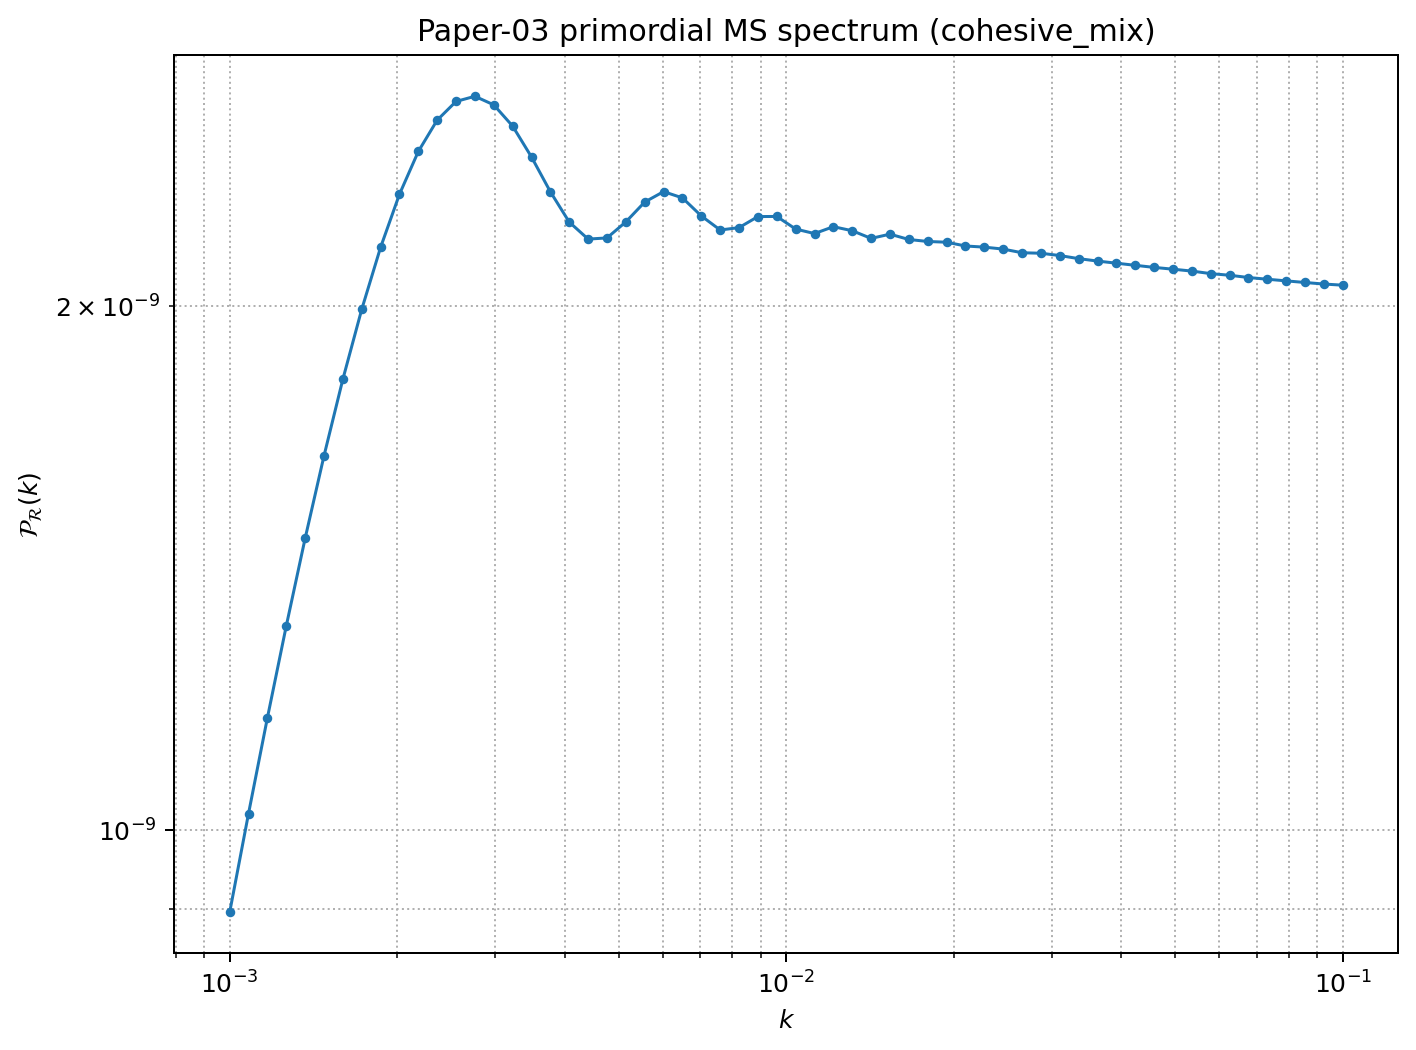
\includegraphics[width=0.72\textwidth]{../figs/primordial_ms_spectrum.png}
  \caption{Primordial scalar spectrum generated by the Paper~III MS pipeline (\texttt{compute\_ms\_spectrum.py}) for the cohesive-mixture benchmark.}
  \label{fig:ms-spectrum}
\end{figure}

% ----------------------------------------
\section{Primordial observables and benchmark windows}
\label{sec:observables}
% ----------------------------------------

From the computed spectra we extract baseline observables:
\begin{equation}
(n_s,\,A_s,\,r,\,\alpha_s),
\end{equation}
within explicitly stated benchmark windows.
For the current scalar-only benchmark run, we obtain
\begin{align}
A_s &\simeq 2.1\times10^{-9},\\
n_s &\simeq 0.9643\quad\text{(local fit around }k_{\rm pivot}=0.05\text{)},\\
\alpha_s &\simeq -1.43\times10^{-3},
\end{align}
with $r$ not extracted at this stage by the scalar-only script.
The difference between $n_s^{\rm MS}$ and the quoted local-fit value reflects two different estimators: a global fit over the full $k$ range versus a local polynomial fit around the pivot, the latter being the quantity propagated to the CLASS external-spectrum bridge.
In the current script the local quadratic fit uses the 35 points closest to $k_{\rm pivot}$ (configurable with \texttt{--fit-window}).

\begin{table}[t]
  \centering
  \begin{tabular}{lc}
    \hline\hline
    Observable & Benchmark value \\
    \hline
    $A_s$ & $2.1\times10^{-9}$ \\
    $n_s$ (local fit) & $0.9643$ \\
    $\alpha_s$ (quadratic fit) & $-1.43\times10^{-3}$ \\
    $r$ & not extracted in scalar-only run \\
    \hline\hline
  \end{tabular}
  \caption{Paper~III baseline primordial observables for the current benchmark.}
  \label{tab:paper3-observables}
\end{table}

\begin{figure}[t]
  \centering
  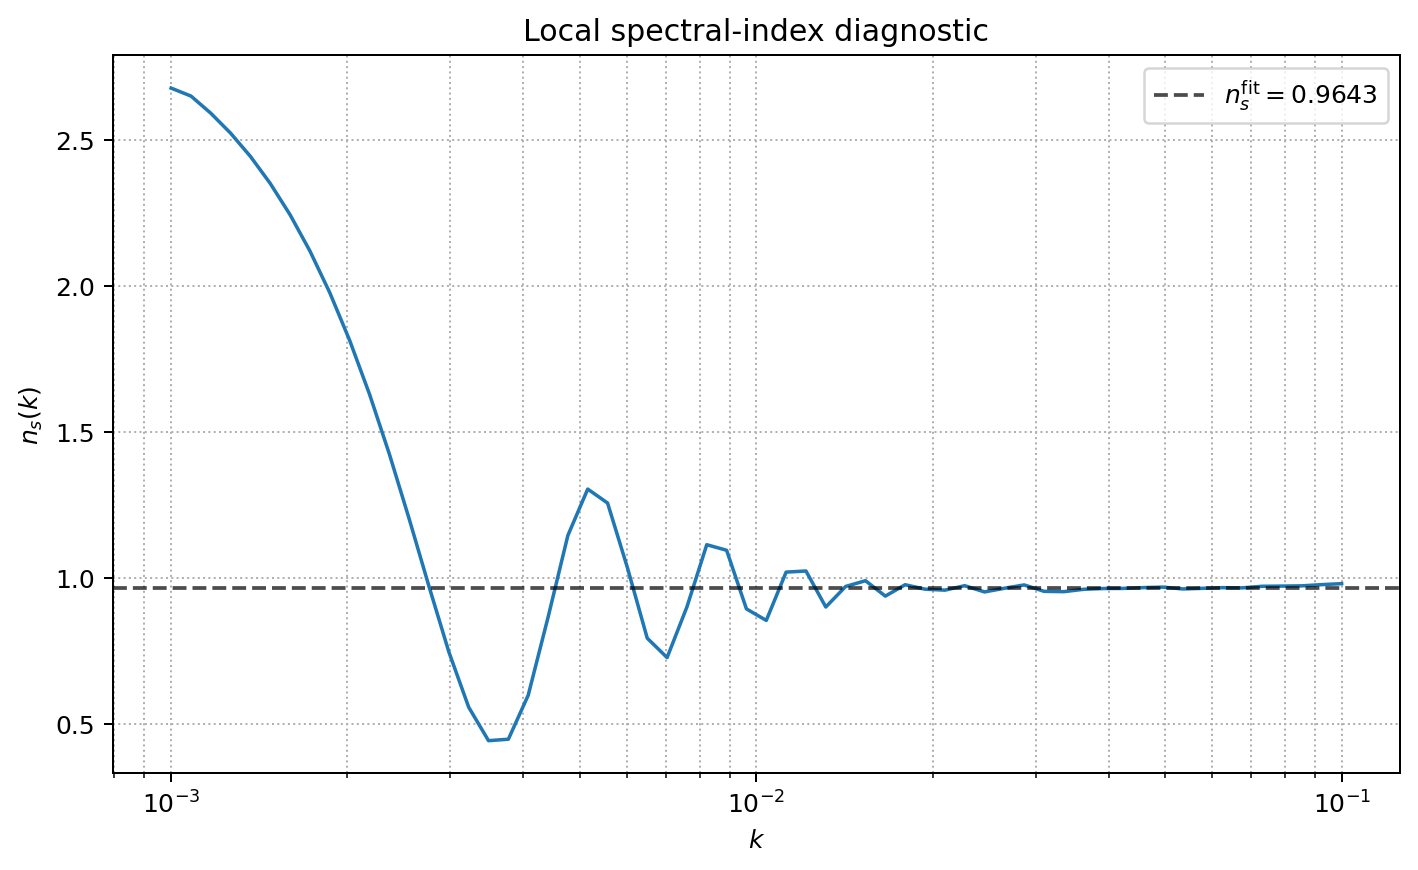
\includegraphics[width=0.72\textwidth]{../figs/primordial_observables_diagnostics.png}
  \caption{Local spectral-index diagnostic derived from the tabulated primordial spectrum (\texttt{compute\_primordial\_observables.py}).}
  \label{fig:primordial-observables}
\end{figure}

% ----------------------------------------
\section{CLASS/CAMB bridge status and consistency checks}
\label{sec:bridge}
% ----------------------------------------

Tabulated primordial spectra are passed to the shared TCV-$\phi$ Boltzmann interface.
In this paper, these runs are used as reproducibility and consistency checks.
A full data-level likelihood analysis is deferred to dedicated follow-up work.
In the present benchmark, CLASS runs in both modes (power-law and external table) complete without fallback, and the ratio of reconstructed matter spectra remains close to unity:
\begin{equation}
0.9988 \lesssim \frac{P_{\rm external}(k)}{P_{\rm powerlaw}(k)} \lesssim 1.0014.
\end{equation}
This confirms interface-level consistency of the exported primordial table for the chosen benchmark.
CAMB runs are not included in the present benchmark script and are left to a dedicated follow-up implementation.

\begin{figure}[t]
  \centering
  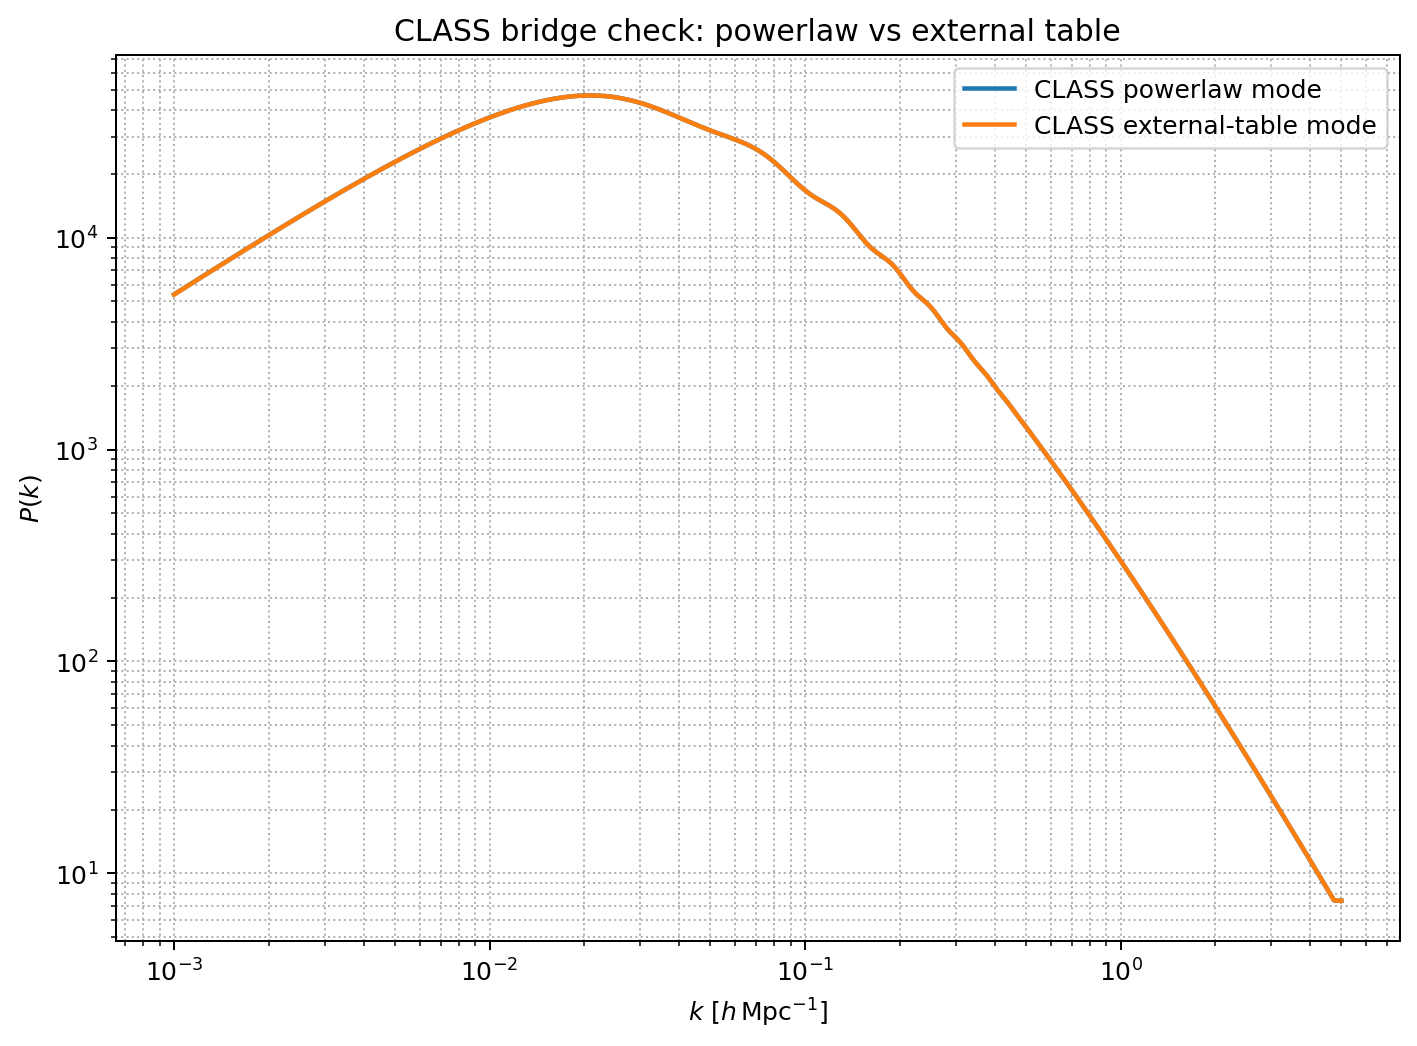
\includegraphics[width=0.72\textwidth]{../figs/class_bridge_pk_comparison.png}
  \caption{CLASS bridge consistency check: power-law mode versus external primordial-table mode.}
  \label{fig:class-bridge-comparison}
\end{figure}

\begin{figure}[t]
  \centering
  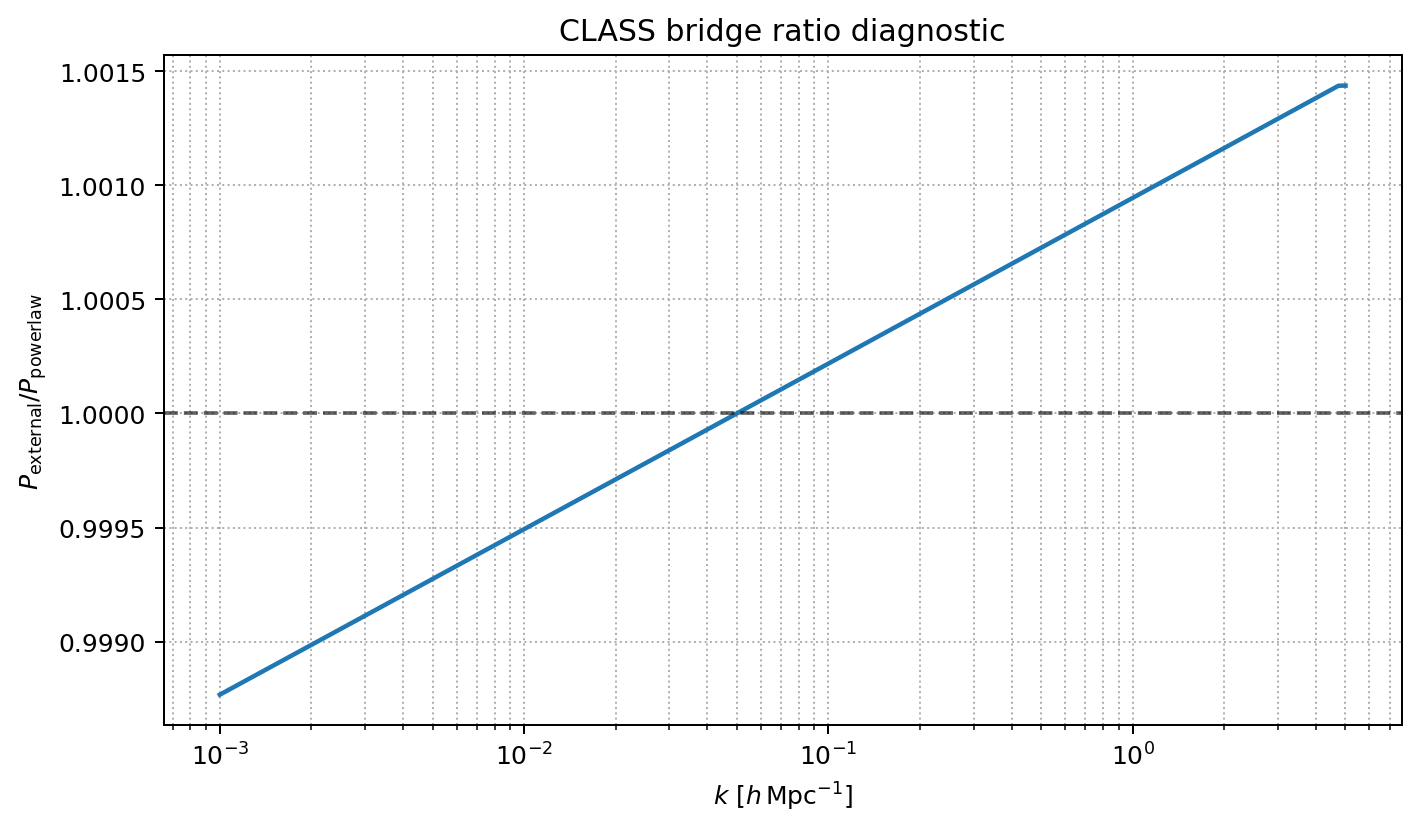
\includegraphics[width=0.72\textwidth]{../figs/class_bridge_pk_ratio.png}
  \caption{Ratio diagnostic for the CLASS bridge test. The near-unity ratio is expected for the matched benchmark setup and validates table-mode reproducibility.}
  \label{fig:class-bridge-ratio}
\end{figure}

% ----------------------------------------
\section{Status of assumptions and outlook}
\label{sec:status}
% ----------------------------------------

This paper keeps the same tiered status labelling as Papers I and II:
\begin{itemize}[leftmargin=1.5em]
  \item EFT-derived equations and definitions;
  \item phenomenological closure ans\"atze used for numerical completion;
  \item deferred sectors for later papers (e.g. full strong-gravity BH analysis in Paper IV).
\end{itemize}
To keep parameter consistency explicit across papers, each run writes a JSON summary that stores both
(i) canonical Paper~I CLASS/CAMB inputs and (ii) the Paper~III ansatz controls used by the MS solver.

% ----------------------------------------
\section{Conclusion}
% ----------------------------------------

Paper III delivers the primordial perturbation layer of the TCV-$\phi$ programme in a reproducible PRD-ready format.
The results are presented conservatively, with explicit diagnostics and without claims beyond the demonstrated benchmark scope.

% ----------------------------------------
% Bibliography placeholder
% ----------------------------------------
\begin{thebibliography}{99}

\bibitem{TCV1}
C.~Lecroq,
``TCV-$\phi$ I: an effective cohesive--vacuum field theory and its $\Lambda$CDM--compatible background cosmology,''
preprint (2026),  \href{https://doi.org/10.5281/zenodo.19234640}{zenodo.19234640}.

\bibitem{TCV2}
C.~Lecroq,
``TCV-$\phi$ II: cohesive bounce, geometric reheating, and baseline baryogenesis/ULDM pipelines,''
preprint (2026), \href{https://doi.org/10.5281/zenodo.19234953}{zenodo.19234953}.

\end{thebibliography}

\end{document}
